\chapter{Исследовательская часть}

В данной части будет проведен анализ времени отрисовки кадра при различных входных данных.

\section{Технические характеристики}

Технические характеристики устройства, на котором выполнялось исследование представлены далее:

\begin{enumerate}[label=\arabic*)]
	\item операционная система --- Ubuntu 22.04.3~\cite{ubuntu} Linux x86\_64;
	\item память --- 16 Гб;
	\item процессор --- Intel® Core™ i5-1135G7 @ 2.40 ГГц.
\end{enumerate}

\section{Время генерации кадра}

Используются функции замера процессорного времени \textit{$std::chrono::system\_clock::now(...)$} и \textit{$std::chrono::duration\_cast<std::chrono::milliseconds>$} из библиотеки $chrono$ на \textit{C++}. Функция возвращает процессорное время в миллисекундах.

Замеры проводились для разного количества фламинго на сцене --- от 1 до 15 и для разного количества источников света --- от 1 до 10.

Результаты замеров времени приведены в таблицах~\ref{tbl:time1} и \ref{tbl:time2} (время в мс). А их графическое представление на рисунках~\ref{fig:graph_3d}~и~\ref{fig:graph_up} соответсвенно.

\begin{table}[htbp]
	\centering
	\caption{Результаты замеров времени (1-5 источников света)}
	\label{tbl:time1}
	\begin{tabular}{|p{2cm}|c|c|c|c|c|c|c|c|c|}
		\hline
		Кол-во & \multicolumn{5}{c|}{Количество источников света} \\ \cline{2-6} 
		фламинго & 1 & 2 & 3 & 4 & 5 \\ \hline
		1 & 325.04 & 483.8 & 612.4 & 951.4 & 1169.04 \\ \hline
		2 & 347.562 & 515.552 & 704.496 & 979.096 & 1196.68 \\ \hline
		3 & 359.622 & 536.262 & 767.9 & 1041.52 & 1232.87 \\ \hline
		4 & 374.705 & 564.41 & 797.116 & 1081.74 & 1268.95 \\ \hline
		5 & 386.948 & 581.216 & 818.725 & 1118.27 & 1428.08 \\ \hline
		6 & 401.118 & 646.689 & 855.869 & 1148.33 & 1318.48 \\ \hline
		7 & 414.805 & 682.748 & 932.195 & 1182.57 & 1425.22 \\ \hline
		8 & 431.992 & 703.39 & 917.808 & 1246.54 & 1537.09 \\ \hline
		9 & 493.04 & 722.936 & 1045.51 & 1279.62 & 1544.96 \\ \hline
		10 & 496.762 & 757.037 & 1084.02 & 1292.98 & 1568.52 \\ \hline
		11 & 509.95 & 775.841 & 1184.6 & 1353.12 & 1577.66 \\ \hline
		12 & 522.278 & 804.074 & 1152.9 & 1418.92 & 1746.19 \\ \hline
		13 & 539.571 & 847.923 & 1185.88 & 1444.88 & 1738.25 \\ \hline
		14 & 556.383 & 887.557 & 1212.68 & 1494.04 & 1747.57 \\ \hline
		15 & 570.041 & 910.32 & 1250.13 & 1532.452 & 1790.42 \\ \hline
	\end{tabular}
\end{table}

\begin{table}[htbp]
	\centering
	\caption{Результаты замеров времени (6-10 источников света)}
	\label{tbl:time2}
	\begin{tabular}{|p{2cm}|c|c|c|c|c|c|c|c|c|}
		\hline
		Кол-во & \multicolumn{5}{c|}{Количество источников света} \\ \cline{2-6} 
		фламинго & 6 & 7 & 8 & 9 & 10 \\ \hline
		1 & 1248.68 & 1539.35 & 1734.08 & 1789.25 & 496.762 \\ \hline
		2 & 1304.91 & 1603.49 & 1740 & 1885.53 & 757.037 \\ \hline
		3 & 1349.08 & 1625.62 & 1782.72 & 2016.54 & 1084.02 \\ \hline
		4 & 1396.44 & 1651.1 & 1860.19 & 2185.9 & 1152.9 \\ \hline
		5 & 1457.22 & 1702.88 & 1914.93 & 2275.28 & 1185.88 \\ \hline
		6 & 1509.89 & 1765.72 & 1981.04 & 2318.69 & 1318.48 \\ \hline
		7 & 1569.4 & 1830.79 & 2054.04 & 2387.47 & 1425.22 \\ \hline
		8 & 1639.82 & 1889.27 & 2154.76 & 2416.02 & 1537.09 \\ \hline
		9 & 1685.39 & 1952.49 & 2224.71 & 2554.56 & 1544.96 \\ \hline
		10 & 1730.46 & 2046.66 & 2273.11 & 2614.62 & 1568.52 \\ \hline
		11 & 1783.34 & 2084.91 & 2339.2 & 2796.38 & 1577.66 \\ \hline
		12 & 1824.53 & 2126.68 & 2492.73 & 2862.62 & 1746.19 \\ \hline
		13 & 1881.78 & 2209.03 & 2558.71 & 3029.14 & 1738.25 \\ \hline
		14 & 1921.89 & 2265.88 & 2635.27 & 3113.45 & 1747.57 \\ \hline
		15 & 1979.87 & 2312.32 & 2698.32 & 3212.42 & 1790.42 \\ \hline
	\end{tabular}
\end{table}

\begin{figure}[h!]
	\centering
	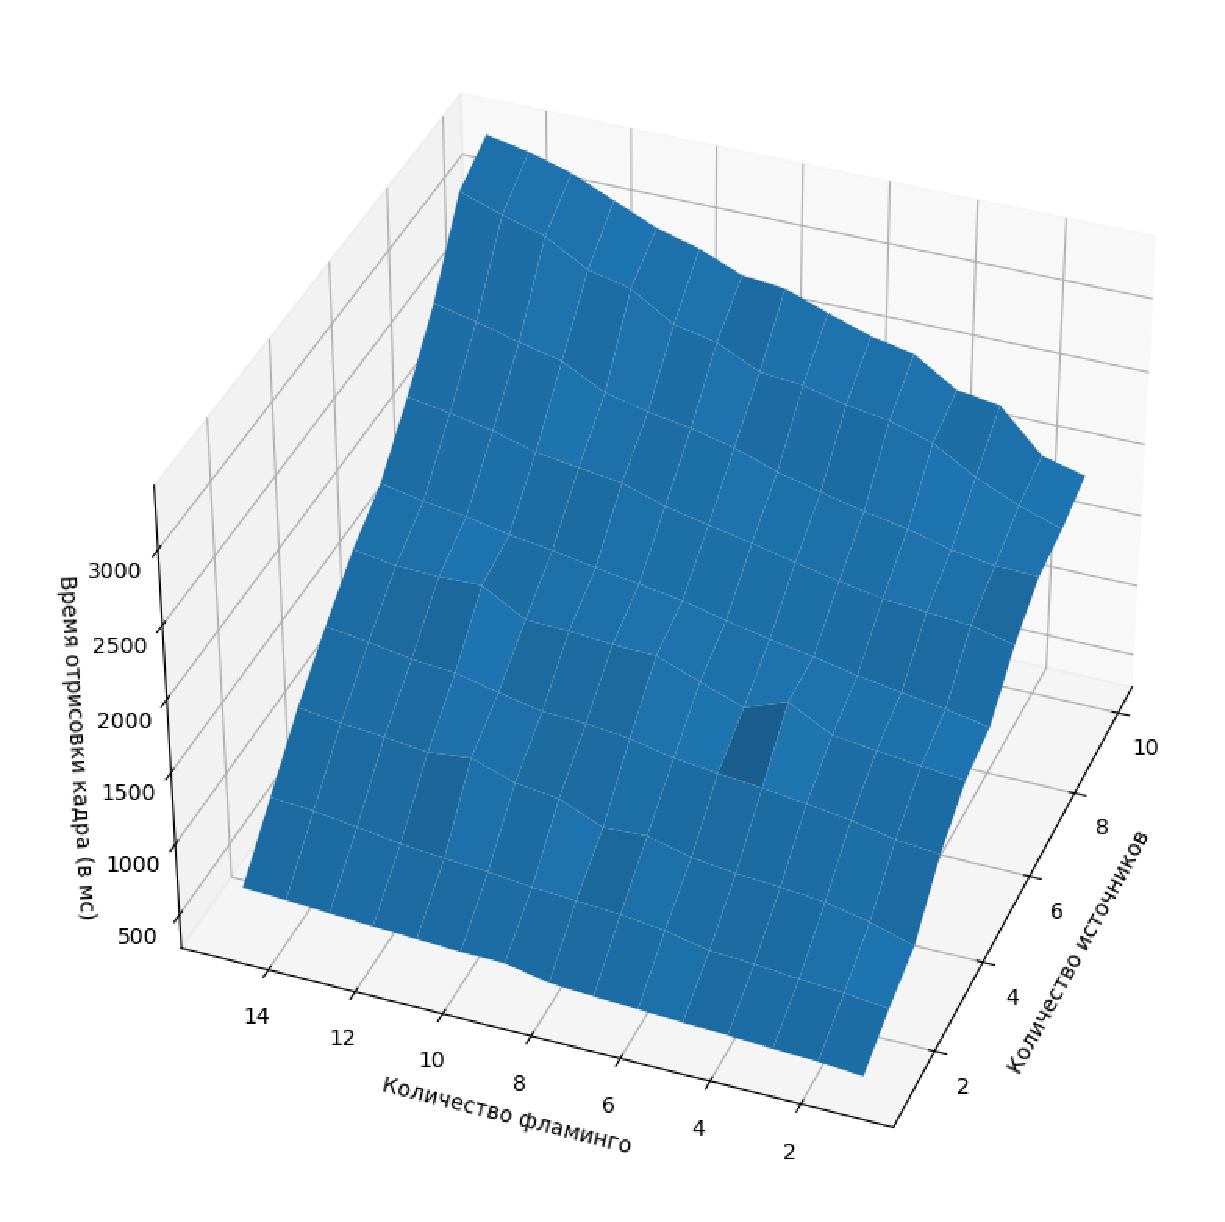
\includegraphics[width=0.7\linewidth]{img/graph_3d}
	\caption{Сравнение времени отрисовки кадра при разном количестве фламинго и источников света}
	\label{fig:graph_3d}
\end{figure}

\begin{figure}[h!]
	\centering
	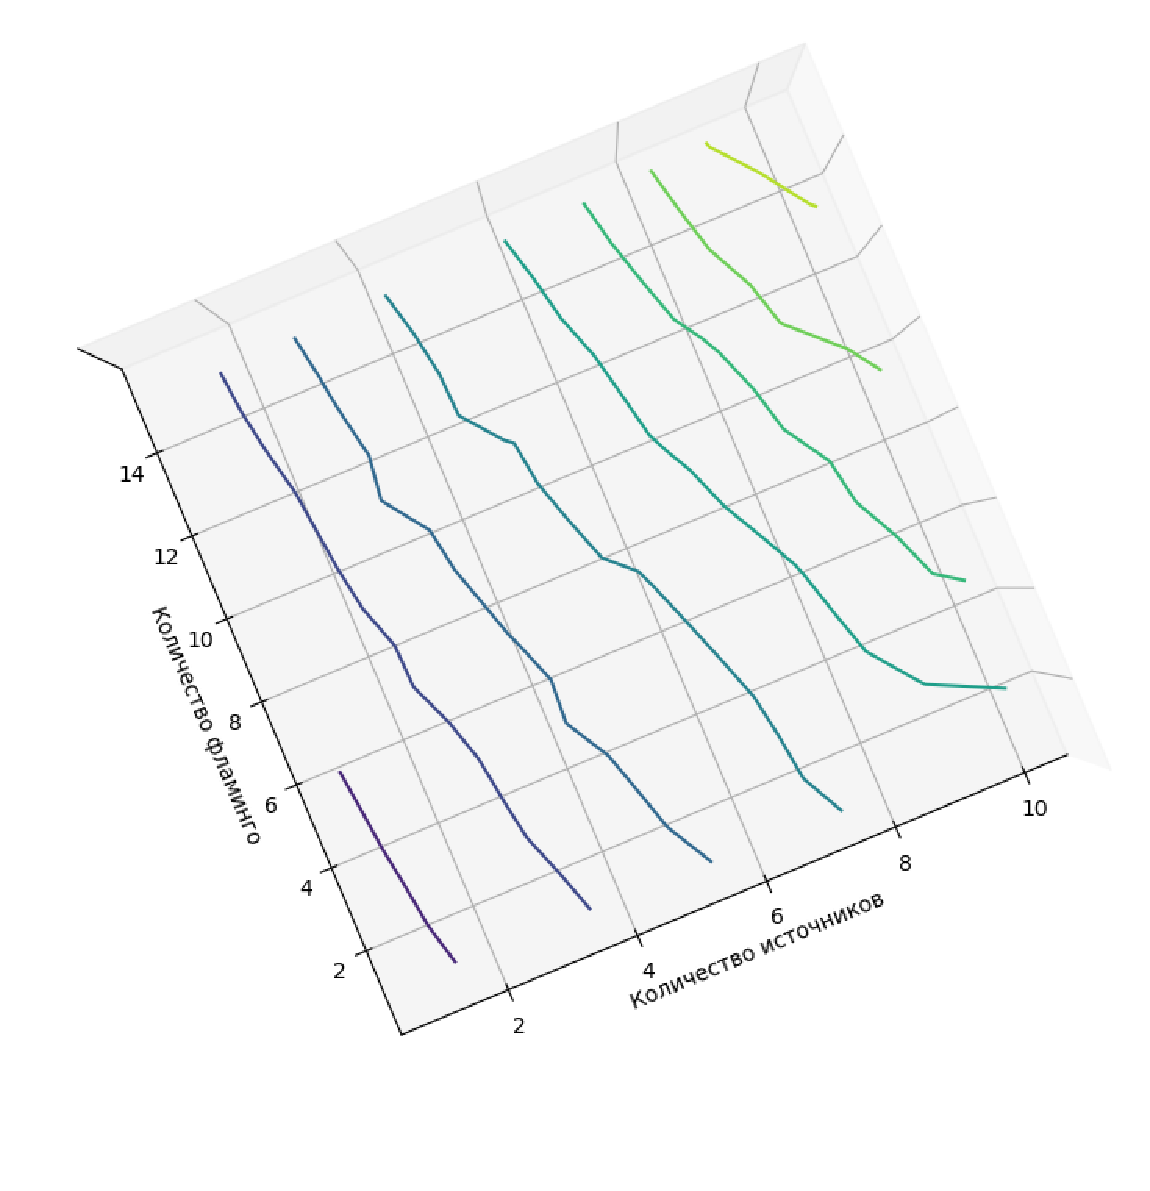
\includegraphics[width=0.6\linewidth]{img/graph_up}
	\caption{Линии уровня графика сравнения времени отрисовки кадра при разном количестве фламинго и источников света}
	\label{fig:graph_up}
\end{figure}
\clearpage

Эта функция зависимости времение от количества фламинго и источников света на сцене можно аппроксимируется функцией~(\ref{for:appr}).

\begin{equation}
	\label{for:appr}
	f(x, y) = 0.833 \cdot y^2 + 0.038 \cdot x^2 + 8.598 \cdot x \cdot y + 169.857 \cdot y + 8.693 \cdot x + 153.645,
\end{equation}
где $x$ --- количество фламинго, $y$ --- количество источников света, $f(x, y)$ --- функция зависимости времени.

На рисунке~\ref{fig:appr} изображены исходные точки синим цветом и аппроксимирущая поверхность, заданная функцией~(\ref{for:appr}), зеленым цветом.

\begin{figure}[h!]
	\centering
	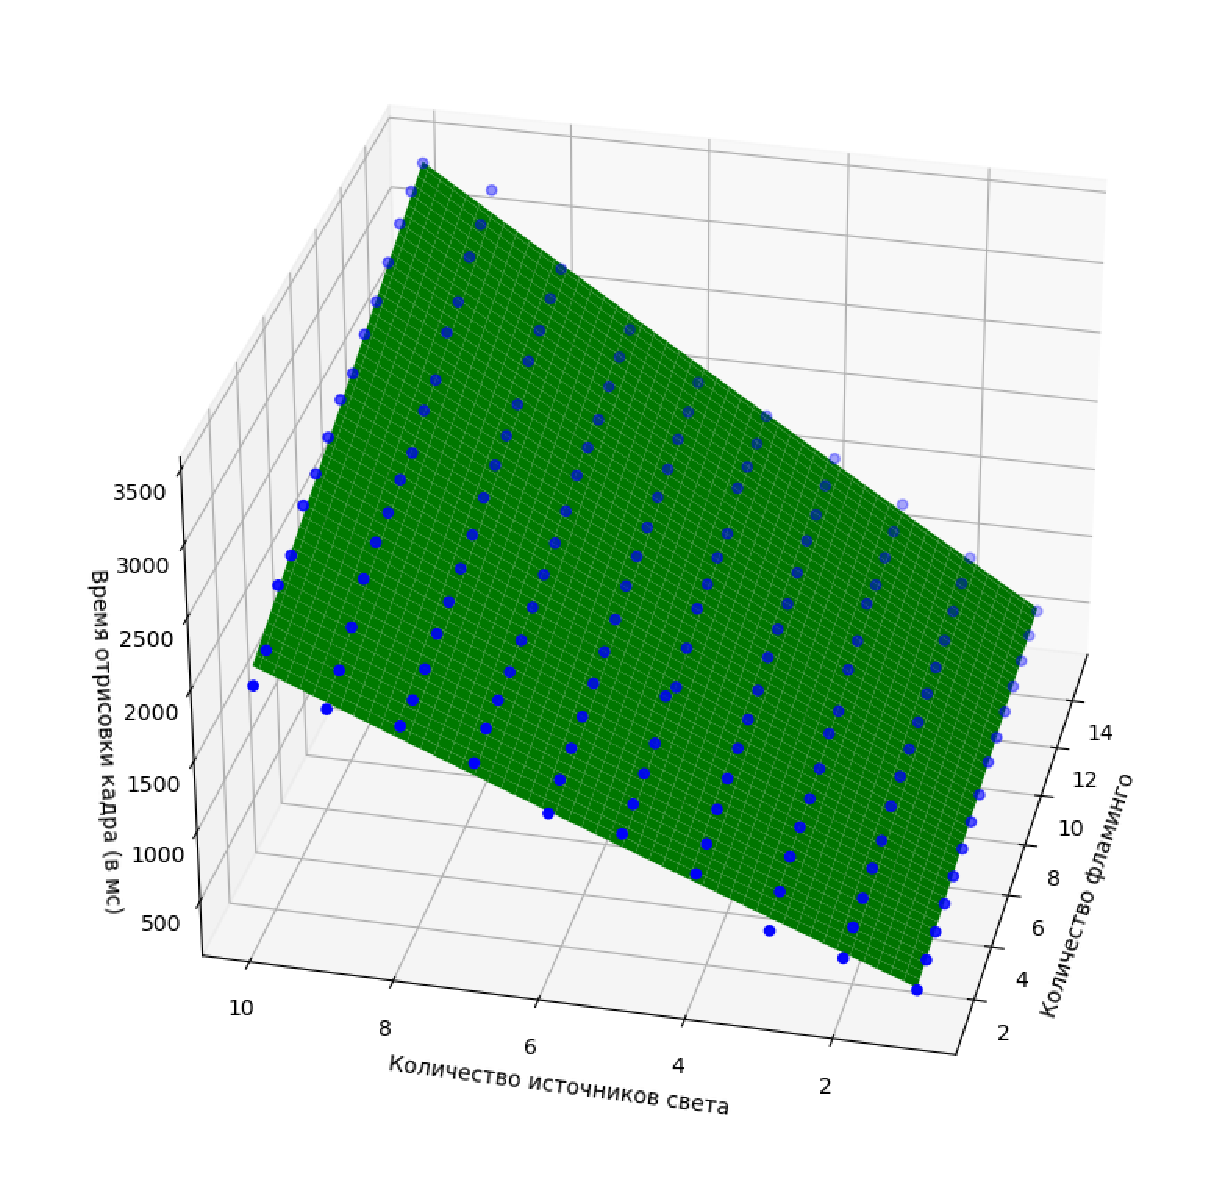
\includegraphics[width=0.75\linewidth]{img/appr}
	\caption{Аппроксимирующая поверхность}
	\label{fig:appr}
\end{figure}

\section{Выводы к исследовательской части}

В данной части был проведен сравнительный анализ времени выполнения работы программы для отрисовки 1 кадра при различном количестве фламинго и источников света на сцене. Из проведенного эксперимента можно сделать вывод, что функция зависимости времени от количества фламинго и источников света на сцене является полиномом 2 степени. При минимальном количестве фламинго и источников света время отрисовки кадра равняется примерно 0.3 секунды, а при 10 фламинго и 10 источников света время становится уже около 1.5 секунд.